\documentclass{beamer}

% For more theme options:
%/usr/share/texmf/tex/latex/beamer/base/themes/theme/compatibility
\usepackage{beamerthemelined}

% this package seems to throw an error for me. -Juneki 12/6/14
%\usepackage[usenames,dvipsnames,svgnames,table]{xcolor}
\usepackage{soul}

\usepackage{algorithm}
\usepackage[noend]{algpseudocode}
\usepackage{graphicx}
\usepackage{caption}
\usepackage{subcaption}
\usepackage{longtable}

\usepackage{tikz-dependency}

\newcommand{\eqnref}[1]{\eqref{eqn:#1}}
%\usepackage[usenames,dvipsnames,svgnames,table]{xcolor}  % allows better color names
\usepackage{todonotes}   % insert [disable] to disable all notes
\newcommand{\Note}[4][]{\todo[author=#2,color=#3,fancyline,#1]{#4}}
\newcommand{\noteJH}[2][]{\Note[#1]{JH}{blue!40}{#2}}
\newcommand{\noteJE}[2][]{\Note[#1]{JE}{green!40}{#2}}
\newcommand{\notewho}[3][]{\Note[#1]{#2}{orange!40}{#3}}  % extra arg with miscellaneous author
\newcommand{\NoteJH}[2][]{\noteJH[inline,#1]{#2}}
\newcommand{\NoteJE}[2][]{\noteJE[inline,#1]{#2}}
\newcommand{\Notewho}[3][]{\notewho[inline,#1]{#2}{#3}}  % extra arg with miscellaneous author


\setbeamerfont{page number in head/foot}{}
\setbeamertemplate{footline}[frame number]

\begin{document}
\title{Deriving Multi-Headed Planar Dependency Parses from Link Grammar Parses}
\author{Juneki Hong, Jason Eisner}
\date{\today}
\frame{\titlepage} %\NoteJH{Include pictures of us?}

\section{Motivation}

\frame{\frametitle{Single-headedness}
  Dependency parse treebanks today are single-headed.


\begin{figure}
  \begin{dependency}
	\begin{deptext}
	  {\scriptsize DT} \& {\scriptsize NN} \& {\scriptsize MD} \& {\scriptsize RB} \& {\scriptsize RB} \& {\scriptsize VB} \& {\scriptsize VB} \& {\scriptsize IN} \& {\scriptsize NN} \& {\scriptsize .} \\
	  the \& matter \& may \& never \& even \& be \& tried \& in \& court \& . \\
	\end{deptext}
	\deproot[edge above, thick, edge style = {blue}]{3}{\small ROOT}
	\depedge[edge above, thick, edge style = {blue}]{3}{2}{\small SBJ}
	\depedge[edge above, thick, edge style = {blue}]{3}{4}{\small ADV}
	\depedge[edge above, thick, edge style = {blue}]{3}{5}{\small ADV}
	\depedge[edge above, thick, edge style = {blue}]{3}{6}{\small VC}
	\depedge[edge above, thick, edge style = {blue}, edge unit distance =1.5ex]{3}{10}{\small P}
	\depedge[edge above, thick, edge style = {blue}]{2}{1}{\small NMOD}
	\depedge[edge above, thick, edge style = {blue}]{7}{8}{\small ADV}
	\depedge[edge above, thick, edge style = {blue}]{6}{7}{\small VC}
	\depedge[edge above, thick, edge style = {blue}]{8}{9}{\small PMOD}
  \end{dependency}
  \caption*{Some example dependency parse.}
\end{figure}

}

%\subsection{Multi-headed}
\frame{\frametitle{Multi-headedness}
  Multi-headedness Can Capture Additional Linguistic Phenomenon
  \begin{itemize}
    \item Control
    \item Relativization
    \item Conjunction
  \end{itemize}
}

\subsection{Control}
\frame{\frametitle{Control}
  \begin{figure}
    \begin{dependency}
      \begin{deptext}
        Jill \& likes \& to \& skip \\
      \end{deptext}
      \deproot[edge above, thick, hide label, edge unit distance = 1.5ex]{2}{}
      \depedge[edge above, thick, hide label]{2}{1}{}
      \depedge[edge below, ultra thick, hide label, edge style = {purple}, edge unit distance = 1.2ex]{4}{1}{}
      \depedge[edge above, thick, hide label]{2}{3}{}
      \depedge[edge above, thick, hide label]{3}{4}{}
    \end{dependency}
    \caption*{Jill is the subject of two verbs}
  \end{figure}

  \begin{figure}
    \begin{dependency}
      \begin{deptext}
        Jill \& persuaded \& Jack \& to \& skip \\
      \end{deptext}
      \deproot[edge above, thick, hide label, edge unit distance = 1.5ex]{2}{}
      \depedge[edge above, thick, hide label]{2}{1}{}
      \depedge[edge above, thick, hide label]{2}{3}{}
      \depedge[edge above, thick, hide label]{3}{4}{}
      \depedge[edge above, thick, hide label]{4}{5}{}
      \depedge[edge below, ultra thick, hide label, edge style = {purple}, edge unit distance = 1.5ex]{3}{5}{}
    \end{dependency}
    \caption*{Jack is the object of one verb and the subject of another}
  \end{figure}
}


\subsection{Relativization}
\frame{\frametitle{Relativization}
  \begin{figure}
    \begin{dependency}
      \begin{deptext}
        The \& boy \& that \& Jill \& skipped \& with \& fell \& down \\
      \end{deptext}
      \deproot[edge above, thick, hide label, edge unit distance = 2ex]{7}{}
      \depedge[edge above, thick, hide label]{2}{1}{}
      \depedge[edge above, thick, hide label]{2}{3}{}
      \depedge[edge above, thick, hide label]{3}{5}{}
      \depedge[edge above, thick, hide label]{5}{4}{}
      \depedge[edge above, thick, hide label]{5}{6}{}
      \depedge[edge above, thick, hide label, edge unit distance = 1.8ex]{7}{2}{}
      \depedge[edge above, thick, hide label]{7}{8}{}
      \depedge[edge below, ultra thick, hide label, edge style = {purple}, edge unit distance = 1.5ex]{6}{2}{}
    \end{dependency}
    \caption*{The boy is the object of \textit{with} as well as the subject of \textit{fell}.}
  \end{figure}
}


\subsection{Conjunction}
\frame{\frametitle{Conjunction}
  \begin{figure}
    \begin{dependency}
      \begin{deptext}
        Jack \& and \& Jill \& went \& up \& the \& hill \\
      \end{deptext}
      \deproot[edge above, thick, hide label, edge unit distance = 2ex]{4}{}
      \depedge[edge above, thick, hide label]{2}{1}{}
      \depedge[edge above, thick, hide label]{2}{3}{}
      \depedge[edge above, thick, hide label]{4}{2}{}
      \depedge[edge above, thick, hide label]{4}{5}{}
      \depedge[edge above, thick, hide label]{5}{7}{}
      \depedge[edge above, thick, hide label]{7}{6}{}

      \depedge[edge below, ultra thick, hide label, edge style = {purple}, edge unit distance = 1.5ex]{4}{1}{}
      \depedge[edge below, ultra thick, hide label, edge style = {purple}, edge unit distance = 1.5ex]{4}{3}{}

    \end{dependency}
    \caption*{Jack and Jill serve as the two arguments to \textit{and}, but are also subjects of \textit{went}.}
  \end{figure}
}



\subsection{Motivation}
\frame{\frametitle{Motivation}
  \begin{itemize}
    \uncover<1->{\item A multiheaded dependency corpus would be useful for testing new parsing algorithms}
    \uncover<2->{\item Such a corpus could be automatically annotated using Integer Linear Programming}
    \uncover<3->{\item We explored whether the Link Grammar could be adapted for this purpose.}
    \uncover<4->{\item The results of this are mixed, but provides a good case study.}
  \end{itemize}
}







% Shouldn't mention non-projectivity. 
%\frame{\frametitle{Non-projectivity}
%\begin{figure}
%  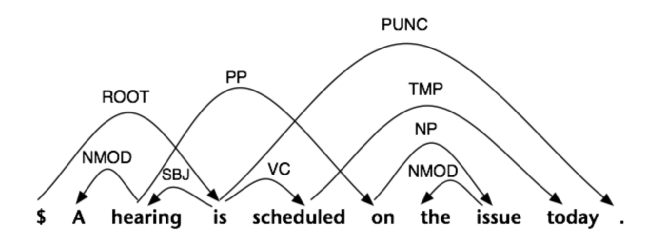
\includegraphics[width=\linewidth]{multiheaded}
%  \caption*{English is not a completely projective language}
%  \NoteJH{image taken from Chris Dyer's slide: http://demo.clab.cs.cmu.edu/fa2014-11711/images/0/0e/Depparsing.pdf}
%  \NoteJH{I should also ask Chris for permission to use this}
%\end{figure}
%}


%\section{Non Projectivity}
%\frame{\frametitle{We do not address: Non-Projectivity}
%\begin{itemize}
%  \item Projectivity assumptions allow us to have efficient parsing algorithms that utilize dynamic programming
%  \item English is mostly projective
%\end{itemize}

%\NoteJH{Should I mention non-projectivity? This slide is mostly here because of a reviewer comment.}
%}

%\frame{\frametitle{We do not address: Non-Projectivity}
%\begin{itemize}
%  \item Projectivity assumptions allow us to have efficient parsing algorithms that utilize dynamic programming
%  \item English is mostly projective
%\end{itemize}

%\begin{figure}
%  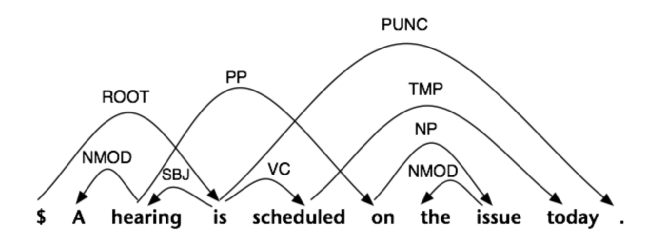
\includegraphics[width=0.7\linewidth]{multiheaded}
%  \caption*{But not always}
%  \NoteJH{image taken from Chris Dyer's slide: http://demo.clab.cs.cmu.edu/fa2014-11711/images/0/0e/Depparsing.pdf}
%  \NoteJH{I should also ask Chris for permission to use this}
%\end{figure}


%}


\section{Link Grammars}

\frame{\frametitle{Link Grammars}
  \begin{itemize}
    \item[] Grammar-based formalism for projective dependency parsing with undirected links
  \end{itemize}
}

\frame{\frametitle{Link Grammars: Example Parse}
  \begin{figure}
    \begin{dependency}[edge style={-}]
	  \begin{deptext}
	    - \& n-u \& v \& e \& e \& v \& v-d \& r \& n-u \& - \\
	    the \& matter \& may \& never \& even \& be \& tried \& in \& court \& . \\
	  \end{deptext}
	  \depedge[edge above, thick, edge style = {red}]{2}{3}{S}
	  \depedge[edge above, thick, edge style = {red}]{3}{6}{I}
	  \depedge[edge above, thick, edge style = {red}]{2}{1}{D}
	  \depedge[edge above, thick, edge style = {red}]{7}{8}{MV}
	  \depedge[edge above, thick, edge style = {red}]{6}{7}{P}
	  \depedge[edge above, thick, edge style = {red}]{8}{9}{J}
	  \deproot[edge above, thick, edge style = {red}]{2}{W}
	  \deproot[edge above, thick, edge style = {red}]{7}{WV}
	  \deproot[edge above, thick, edge style = {red}]{10}{X}
	  \depedge[edge above, thick, edge style = {red}]{6}{4}{E}
	  \depedge[edge above, thick, edge style = {red}]{6}{5}{E}
    \end{dependency}
    \caption*{Link Parse of a sentence from Penn Tree Bank}
  \end{figure}
}

\frame{\frametitle{Link Grammars: Converting into a Directed Acyclic Graph}
  \begin{figure}
    \begin{dependency}
	  \begin{deptext}
	    - \& n-u \& v \& e \& e \& v \& v-d \& r \& n-u \& - \\
	    the \& matter \& may \& never \& even \& be \& tried \& in \& court \& . \\
	  \end{deptext}
	  \depedge[edge above, thick, edge style = {red}]{2}{3}{S}
	  \depedge[edge above, thick, edge style = {red}]{3}{6}{I}
	  \depedge[edge above, thick, edge style = {red}]{2}{1}{D}
	  \depedge[edge above, thick, edge style = {red}]{7}{8}{MV}
	  \depedge[edge above, thick, edge style = {red}]{6}{7}{P}
	  \depedge[edge above, thick, edge style = {red}]{8}{9}{J}
	  \deproot[edge above, thick, edge style = {red}]{2}{W}
	  \deproot[edge above, thick, edge style = {red}]{7}{WV}
	  \deproot[edge above, thick, edge style = {red}]{10}{X}
	  \depedge[edge above, thick, edge style = {red}]{6}{4}{E}
	  \depedge[edge above, thick, edge style = {red}]{6}{5}{E}
    \end{dependency}
    
    \caption*{Directionalize the edges}
  \end{figure} 
}


\frame{\frametitle{Link Grammars}
Compare resulting dependency parse with CoNLL 2007 shared task. 
\begin{figure}
  \begin{dependency}
	\begin{deptext}
	  - \& n-u \& v \& e \& e \& v \& v-d \& r \& n-u \& - \\
	  the \& matter \& may \& never \& even \& be \& tried \& in \& court \& . \\
	  {\scriptsize DT} \& {\scriptsize NN} \& {\scriptsize MD} \& {\scriptsize RB} \& {\scriptsize RB} \& {\scriptsize VB} \& {\scriptsize VB} \& {\scriptsize IN} \& {\scriptsize NN} \& {\scriptsize .} \\
	\end{deptext}
	\deproot[edge below, thick, edge style = {blue}]{3}{\small ROOT}
	\depedge[edge above, thick, edge style = {red}]{2}{3}{S}
	\depedge[edge below, thick, edge style = {blue}]{3}{2}{\small SBJ}
	\depedge[edge below, thick, edge style = {blue}]{3}{4}{\small ADV}
	\depedge[edge below, thick, edge style = {blue}]{3}{5}{\small ADV}
	\depedge[edge above, thick, edge style = {red}]{3}{6}{I}
	\depedge[edge below, thick, edge style = {blue}]{3}{6}{\small VC}
	\depedge[edge below, thick, edge style = {blue}, edge unit distance =1.5ex]{3}{10}{\small P}
	\depedge[edge above, thick, edge style = {red}]{2}{1}{D}
	\depedge[edge below, thick, edge style = {blue}]{2}{1}{\small NMOD}
	\depedge[edge above, thick, edge style = {red}]{7}{8}{MV}
	\depedge[edge below, thick, edge style = {blue}]{7}{8}{\small ADV}
	\depedge[edge above, thick, edge style = {red}]{6}{7}{P}
	\depedge[edge below, thick, edge style = {blue}]{6}{7}{\small VC}
	\depedge[edge above, thick, edge style = {red}]{8}{9}{J}
	\depedge[edge below, thick, edge style = {blue}]{8}{9}{\small PMOD}
	\deproot[edge above, thick, edge style = {red}]{2}{W}
	\deproot[edge above, thick, edge style = {red}]{7}{WV}
	\deproot[edge above, thick, edge style = {red}]{10}{X}
	\depedge[edge above, thick, edge style = {red}]{6}{4}{E}
	\depedge[edge above, thick, edge style = {red}]{6}{5}{E}
  \end{dependency}

  \caption*{Top half is CoNLL. Bottom half is the directionalized link parse.}
\end{figure}


}



\frame{\frametitle{Link Grammars}
Compare resulting dependency parse with CoNLL 2007 shared task. 
\begin{figure}
  \begin{dependency}
	\begin{deptext}
	  - \& n-u \& v \& e \& e \& v \& v-d \& r \& n-u \& - \\
	  the \& matter \& may \& never \& even \& be \& tried \& in \& court \& . \\
	  {\scriptsize DT} \& {\scriptsize NN} \& {\scriptsize MD} \& {\scriptsize RB} \& {\scriptsize RB} \& {\scriptsize VB} \& {\scriptsize VB} \& {\scriptsize IN} \& {\scriptsize NN} \& {\scriptsize .} \\
	\end{deptext}
	\deproot[edge below, edge style = {blue, dotted}]{3}{\small ROOT}
	\depedge[edge above, edge style = {red, ultra thick}]{2}{3}{S}
	\depedge[edge below, edge style = {blue, ultra thick}]{3}{2}{\small SBJ}
	\depedge[edge below, edge style = {blue, dotted}]{3}{4}{\small ADV}
	\depedge[edge below, edge style = {blue, dotted}]{3}{5}{\small ADV}
	\depedge[edge above, edge style = {red, thick}]{3}{6}{I}
	\depedge[edge below, edge style = {blue, thick}]{3}{6}{\small VC}
	\depedge[edge below, edge style = {blue, dotted}, edge unit distance =1.5ex]{3}{10}{\small P}
	\depedge[edge above, edge style = {red, thick}]{2}{1}{D}
	\depedge[edge below, edge style = {blue, thick}]{2}{1}{\small NMOD}
	\depedge[edge above, edge style = {red, thick}]{7}{8}{MV}
	\depedge[edge below, edge style = {blue, thick}]{7}{8}{\small ADV}
	\depedge[edge above, edge style = {orange, thick}]{6}{7}{P}
	\depedge[edge below, edge style = {blue, thick}]{6}{7}{\small VC}
	\depedge[edge above, edge style = {red, thick}]{8}{9}{J}
	\depedge[edge below, edge style = {blue, thick}]{8}{9}{\small PMOD}
	\deproot[edge above, edge style = {red, dotted}]{2}{W}
	\deproot[edge above, edge style = {orange, ultra thick, dotted}]{7}{WV}
	\deproot[edge above, edge style = {red, dotted}]{10}{X}
	\depedge[edge above, edge style = {red, dotted}]{6}{4}{E}
	\depedge[edge above, edge style = {red, dotted}]{6}{5}{E}
  \end{dependency}

  \caption*{Top half is CoNLL. Bottom half is the directionalized link parse.}
\end{figure}


}


%\section{ILP}
%\frame{\frametitle{Integer Linear Programming}

%\NoteJH{Will the audience know about ILP?}

%}


\section{ILP Model}


\frame{\frametitle{Integer Linear Programming Model}

Encoded Constraints:
\begin{itemize}
  \item Connectedness
  \item Acyclicity
  \item Consistency of Directionalized Links
\end{itemize}
}



\frame{\frametitle{Integer Linear Programming Model}

For each sentence, for each edge $i,j$, where $i < j$

\begin{figure}
  \begin{dependency}[edge style={-}]
    \begin{deptext}
      . \& . \& . \& $i$ \& . \& . \& . \& $j$ \& . \& . \& . \\
    \end{deptext}
    \depedge[edge above, thick, edge unit distance = 1.1ex]{4}{8}{L}
  \end{dependency}
\end{figure}



Variables: 
\begin{itemize}
\item[] $x_{ij}, x_{ji} \in \mathbb{Z} \geq 0$: orientation of each link
\item[] $x_{ij} + x_{ji} = 1$

%\item $x_{ij} + x_{ji} = 1$ (A link can only be oriented left or right)

\end{itemize}





%\NoteJH{TODO: Incomplete slide. Need to describe things like depth of the variable, label}
}



\frame{\frametitle{Connectedness, Acyclicity}
\begin{itemize}
  \item[] Connectedness
    \begin{align}
      \sum_u x_{uv} & \geq 1
    \end{align}

  \item[] Acyclicity
    \begin{itemize}
      \item[] Given that node $u$ is the parent of $v$
      \item[] $n_v$: length of the sentence containing node $v$
      \item[] $d_v \in [0, n_v]$: depth of the node from the root of the sentence
    \end{itemize}

    \begin{align}
      (\forall_u)\; d_v + (1 + n_v) \cdot (1 - x_{uv}) & \geq 1+d_u
    \end{align}
\end{itemize}

}


\frame{\frametitle{Consistency of Directionalized Links \onslide<2->{with Slack}}
\begin{itemize}
  \item[] Consistency of Directionalized Links
    \begin{itemize}
      \item[] $r_L, \ell_L \in \{0,1\}$: whether links with label $L$ allowed left/right
    \end{itemize}
    
    \begin{align}\label{direction+slack}
      x_{ij} &\leq r_L \onslide<2->{ + s_{ij}} &
      x_{ji} &\leq \ell_L \onslide<2->{ + s_{ij}}
    \end{align}

    \begin{align}\label{eqn:obj}
      \min \left( \sum_L r_L + \ell_L \right) \onslide<2->{\cdot \frac{N_L}{4} + \sum_{ij}s_{ij}}
    \end{align}

    \onslide<2->{\begin{itemize}
      \item[] $s_{ij} \in \mathbb{R} \geq 0$: slack variable 
      \item[] $N_L$: Number of link tokens with label $L$
    \end{itemize}

    \begin{itemize}
      \item[] Slack allows a few links with label $L$ in disallowed directions
    \end{itemize}
    }

\end{itemize}
}


\section{Experiments and Results}
%\frame{\frametitle{Experiments and Results}
%\begin{itemize}
%  \item 18,577 English sentences with gold CoNLL. 
%  \item 18,577 unlabeled Russian sentences.
%\end{itemize}
%}

\frame{\frametitle{Data Sets}
%\begin{itemize}
%  \item[] 18,577 English sentences with 10,960 connected parses
%  \item[] 18,577 unlabeled Russian sentences with 4,913 connected parses
%\end{itemize}
  
  Data Sets taken from:
  \begin{itemize}
    \item[] CoNLL 2007 Shared Task (English)
    \item[] ACL 2013 Shared Task of Machine Translation (Russian)
  \end{itemize}

  \begin{figure}[h]
    \centering
    \begin{tabular}{|l|l|l|}
      \hline
       & Input Sentences & Output Connected Parses \\ \hline
       English  & 18,577        & 10,960               \\ \hline
       Russian & 18,577        & 4,913                \\ \hline
    \end{tabular}
  \end{figure}
}

\frame{\frametitle{Stability of Results}
  \begin{figure}
    \centering
    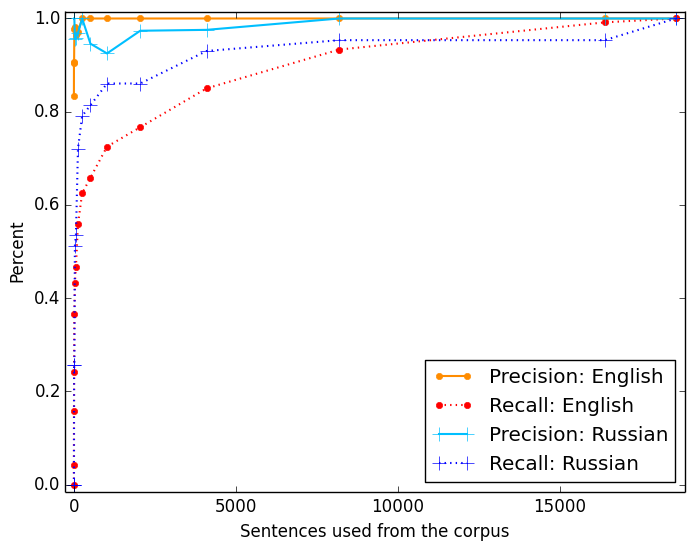
\includegraphics[width=0.7\linewidth]{precision_recall}
  \end{figure}
}



%\frame{\frametitle{On the English data set}
%\begin{itemize}
%\item[] Link Data has 8\% additional edges over the CoNLL.
%\item[] 52\% of links match CoNLL arcs
%\item[] 57\% of CoNLL arcs match links
%\end{itemize}

%
%}

\frame{\frametitle{On the English Data Set:}
  
  \uncover<2->{Multiheadedness}
  \begin{itemize}
  \uncover<2->{\item[] Link Data has 8\% additional edges over the CoNLL.}
  \end{itemize}
  
  \uncover<3->{CoNLL Matches}
  \begin{itemize}
  \uncover<3->{\item[] 52\% of links match CoNLL arcs
  \item[] 57\% of CoNLL arcs match links}
  \end{itemize}

  \uncover<4->{Directionality}%\uncover<5->{ is Mostly Consistent!}
  \begin{itemize}
  \uncover<4->{\item[] 6.19\% of link types allowed both directions %($\frac{7}{113}$)
  \item[] 2.07\% of link tokens required disallowed direction via slack %($\frac{4043}{195,000}$)
  }
  \end{itemize}


  %\uncover<4->{The link labels mostly have a consistent direction.}
  %\uncover<5->{\item[] The direction is often the same as CoNLL when there is a corresponding arc}

}



\frame{\frametitle{ILP Results: Top 25 Most Occuring Labels}

  \begin{figure}
    \centering
    \begin{tiny}
\centering
%\begin{longtable}[width=\textwidth]{|l|l|l|l|l|l|}
\begin{tabular}{|l|l|l|l|l|l|}
\hline
Label & Rightward & Multiheaded & CoNLL Match & CoNLL Dir Match\\\hline
%\endhead

\hline
%\endfoot

A & 0\% (0/8501) & 0\% (0/8501) & 84\% (7148/8501) & 98\% (7002/7148)  \\
AN & 0\% (0/9401) & 0\% (0/9401) & 83\% (7825/9401) & 98\% (7639/7825)  \\
B & 100\% (1514/1515) & 61\% (919/1515) & 53\% (806/1515) & 84\% (678/806)  \\
C & 100\% (3272/3272) & 0\% (0/3272) & 3\% (85/3272) & 53\% (45/85)  \\
CO & 0\% (0/2478) & 1\% (32/2478) & 5\% (114/2478) & 68\% (78/114)  \\
CV & 100\% (3237/3237) & 100\% (3237/3237) & 56\% (1827/3237) & 28\% (512/1827)  \\
D & 0\% (56/19535) & 0\% (71/19535) & 85\% (16656/19535) & 100\% (16608/16656)  \\
E & 0\% (0/1897) & 0\% (2/1897) & 67\% (1279/1897) & 99\% (1263/1279)  \\
G & 0\% (0/6061) & 0\% (0/6061) & 70\% (4258/6061) & 96\% (4070/4258)  \\
I & 100\% (5405/5424) & 60\% (3247/5424) & 95\% (5168/5424) & 47\% (2408/5168)  \\
IV & 100\% (1626/1627) & 100\% (1626/1627) & 85\% (1389/1627) & 97\% (1353/1389)  \\
J & 98\% (16400/16673) & 2\% (280/16673) & 87\% (14522/16673) & 97\% (14069/14522)  \\
M & 100\% (9594/9596) & 0\% (16/9596) & 74\% (7124/9596) & 92\% (6583/7124)  \\
MV & 100\% (13375/13376) & 0\% (61/13376) & 51\% (6797/13376) & 98\% (6681/6797)  \\
MX & 100\% (1999/1999) & 4\% (83/1999) & 42\% (836/1999) & 91\% (763/836)  \\
O & 100\% (11027/11028) & 0\% (0/11028) & 81\% (8932/11028) & 96\% (8535/8932)  \\
P & 100\% (3755/3756) & 31\% (1167/3756) & 94\% (3528/3756) & 100\% (3523/3528)  \\
S & 97\% (13138/13520) & 57\% (7662/13520) & 92\% (12476/13520) & 5\% (586/12476)  \\
SJ & 50\% (2736/5468) & 0\% (0/5468) & 69\% (3778/5468) & 93\% (3502/3778)  \\
TO & 100\% (1733/1734) & 0\% (1/1734) & 0\% (5/1734) & 100\% (5/5)  \\
VJ & 51\% (765/1500) & 1\% (8/1500) & 71\% (1059/1500) & 89\% (939/1059)  \\
W & 100\% (10528/10528) & 0\% (5/10528) & 5\% (504/10528) & 46\% (232/504)  \\
WV & 100\% (7563/7563) & 100\% (7557/7563) & 57\% (4345/7563) & 97\% (4214/4345)  \\
X & 80\% (13132/16406) & 5\% (806/16406) & 8\% (1364/16406) & 95\% (1300/1364)  \\
YS & 0\% (0/1645) & 0\% (0/1645) & 98\% (1619/1645) & 0\% (0/1619)  \\
\hline
%\end{longtable}
\end{tabular}
\end{tiny}

  \end{figure}
}

%\frame{\frametitle{ILP Results: Top 25 Most Occuring Labels}
%  \begin{tiny}
\centering
%\begin{longtable}[width=\textwidth]{|l|l|l|l|l|l|}
\begin{tabular}{|l|l|}
\hline
Label & CoNLL Label\\\hline
%\endhead

\hline
%\endfoot

A & NMOD 98\% (7000/7148) \\
AN & NMOD 96\% (7523/7825) \\
B & NMOD 75\% (603/806) \\
C & NMOD 27\% (23/85) \\
CO & NMOD 39\% (44/114) \\
CV & VMOD 52\% (956/1827) \\
D & NMOD 100\% (16629/16656) \\
E & ADV 84\% (1079/1279) \\
G & NMOD 91\% (3868/4258) \\
I & VMOD 53\% (2756/5168) \\
IV & OBJ 70\% (972/1389) \\
J & PMOD 98\% (14240/14522) \\
M & NMOD 82\% (5873/7124) \\
MV & ADV 75\% (5105/6797) \\
MX & NMOD 89\% (741/836) \\
O & OBJ 73\% (6495/8932) \\
P & VC 60\% (2104/3528) \\
S & SBJ 97\% (12150/12476) \\
SJ & COORD 86\% (3240/3778) \\
TO & ADV 40\% (2/5) \\
VJ & COORD 86\% (916/1059) \\
W & P 52\% (262/504) \\
WV & ROOT 97\% (4214/4345) \\
X & P 100\% (1358/1364) \\
YS & NMOD 100\% (1619/1619) \\
\hline
%\end{longtable}
\end{tabular}
\end{tiny}

%}




\frame{\frametitle{Link Results: Subject-Verb links are backwards}
\begin{figure}
  \begin{dependency}
	\begin{deptext}
	  - \& n-u \& v \& e \& e \& v \& v-d \& r \& n-u \& - \\
	  the \& matter \& may \& never \& even \& be \& tried \& in \& court \& . \\
	  {\scriptsize DT} \& {\scriptsize NN} \& {\scriptsize MD} \& {\scriptsize RB} \& {\scriptsize RB} \& {\scriptsize VB} \& {\scriptsize VB} \& {\scriptsize IN} \& {\scriptsize NN} \& {\scriptsize .} \\
	\end{deptext}
	\deproot[edge below, edge style = {blue, dotted}]{3}{\small ROOT}
	\depedge[edge above, edge style = {red, ultra thick}]{2}{3}{S}
	\depedge[edge below, edge style = {blue, ultra thick}]{3}{2}{\small SBJ}
	\depedge[edge below, edge style = {blue, dotted}]{3}{4}{\small ADV}
	\depedge[edge below, edge style = {blue, dotted}]{3}{5}{\small ADV}
	\depedge[edge above, edge style = {red, thick}]{3}{6}{I}
	\depedge[edge below, edge style = {blue, thick}]{3}{6}{\small VC}
	\depedge[edge below, edge style = {blue, dotted}, edge unit distance =1.5ex]{3}{10}{\small P}
	\depedge[edge above, edge style = {red, thick}]{2}{1}{D}
	\depedge[edge below, edge style = {blue, thick}]{2}{1}{\small NMOD}
	\depedge[edge above, edge style = {red, thick}]{7}{8}{MV}
	\depedge[edge below, edge style = {blue, thick}]{7}{8}{\small ADV}
	\depedge[edge above, edge style = {orange, thick}]{6}{7}{P}
	\depedge[edge below, edge style = {blue, thick}]{6}{7}{\small VC}
	\depedge[edge above, edge style = {red, thick}]{8}{9}{J}
	\depedge[edge below, edge style = {blue, thick}]{8}{9}{\small PMOD}
	\deproot[edge above, edge style = {red, dotted}]{2}{W}
	\deproot[edge above, edge style = {orange, ultra thick, dotted}]{7}{WV}
	\deproot[edge above, edge style = {red, dotted}]{10}{X}
	\depedge[edge above, edge style = {red, dotted}]{6}{4}{E}
	\depedge[edge above, edge style = {red, dotted}]{6}{5}{E}
  \end{dependency}
\end{figure}

}



\frame{\frametitle{Link Results: Subject-Verb links are backwards}
\begin{figure}
  \begin{dependency}
	\begin{deptext}
	  - \& n-u \& v \& e \& e \& v \& v-d \& r \& n-u \& - \\
	  the \& matter \& may \& never \& even \& be \& tried \& in \& court \& . \\
	  {\scriptsize DT} \& {\scriptsize NN} \& {\scriptsize MD} \& {\scriptsize RB} \& {\scriptsize RB} \& {\scriptsize VB} \& {\scriptsize VB} \& {\scriptsize IN} \& {\scriptsize NN} \& {\scriptsize .} \\
	\end{deptext}
	\deproot[edge below, edge style = {gray}, hide label]{3}{\small ROOT}
	\depedge[edge above, edge style = {red, ultra thick}]{2}{3}{S}
	\depedge[edge below, edge style = {blue, ultra thick}]{3}{2}{\small SBJ}
	\depedge[edge below, edge style = {gray}, hide label]{3}{4}{\small ADV}
	\depedge[edge below, edge style = {gray}, hide label]{3}{5}{\small ADV}
	\depedge[edge above, edge style = {gray}, hide label]{3}{6}{I}
	\depedge[edge below, edge style = {gray}, hide label]{3}{6}{\small VC}
	\depedge[edge below, , edge style = {gray}, hide label, edge unit distance =1.5ex]{3}{10}{\small P}
	\depedge[edge above, edge style = {gray}, hide label]{2}{1}{D}
	\depedge[edge below, edge style = {gray}, hide label]{2}{1}{\small NMOD}
	\depedge[edge above, edge style = {gray}, hide label]{7}{8}{MV}
    \depedge[edge below, edge style = {gray}, hide label]{7}{8}{\small ADV}
	\depedge[edge above, edge style = {gray}, hide label]{6}{7}{P}
	\depedge[edge below, edge style = {gray}, hide label]{6}{7}{\small VC}
	\depedge[edge above, edge style = {gray}, hide label]{8}{9}{J}
	\depedge[edge below, edge style = {gray}, hide label]{8}{9}{\small PMOD}
	\deproot[edge above, edge style = {gray}, hide label]{2}{W}
    \deproot[edge above, edge style = {gray}, hide label]{7}{WV}
	\deproot[edge above, edge style = {gray}, hide label]{10}{X}
	\depedge[edge above, edge style = {gray}, hide label]{6}{4}{E}
	\depedge[edge above, edge style = {gray}, hide label]{6}{5}{E}
  \end{dependency}
\end{figure}

}


\frame{\frametitle{Link Results: Subject-Verb links are backwards}

\begin{itemize}
\item In our paper we claimed this was due to an inconsistency of the Link Grammar, discovered by our method. 

\end{itemize}

\begin{figure}
  \begin{dependency}
	\begin{deptext}
	  Jill \& wanted \& to \& skip \\
	\end{deptext}
    \deproot[edge above, edge unit distance=2ex]{1}{W}
    \deproot[edge above, edge unit distance=2ex]{2}{WV}
	\depedge[edge above]{2}{1}{S}
	\depedge[edge above]{2}{3}{TO}
	\depedge[edge above]{3}{4}{I}
	\depedge[edge above]{2}{4}{IV}
  \end{dependency}
\end{figure}

%\begin{figure}
%  \begin{dependency}
%	\begin{deptext}
%	  Jill \& persuaded \& him \& to \& skip \\
%	\end{deptext}
%    \deproot[edge above, edge unit distance=2ex]{1}{W}
%    \deproot[edge above, edge unit distance=2ex]{2}{WV}
%	\depedge[edge above]{2}{1}{S}
%	\depedge[edge above]{2}{3}{O}
%	\depedge[edge above]{2}{4}{TO}
%	\depedge[edge above]{4}{5}{I}
%	\depedge[edge above]{2}{5}{IV}
%  \end{dependency}
%\end{figure}

\begin{figure}
  \begin{dependency}
	\begin{deptext}
	  Jill \& thinks \& he \& will \& skip \\
	\end{deptext}
    \deproot[edge above, edge unit distance=2ex]{1}{W}
    \deproot[edge above, edge unit distance=2ex]{2}{WV}
	\depedge[edge above]{1}{2}{S}
	\depedge[edge above]{2}{3}{C}
	\depedge[edge above]{3}{4}{S}
	\depedge[edge above]{4}{5}{I}
	\depedge[edge above]{2}{5}{CV}
  \end{dependency}
\end{figure}



}


\section{Conclusions}
\frame{\frametitle{Conclusions}
  \begin{itemize}
  \item Link Grammar parses can be oriented into connected DAGs
  \item New corpora for building multi-headed dependency parsers
  \item ILP can be used to build or annotate corpora
  \end{itemize}
}


\frame{\frametitle{}
  \begin{itemize}
  \item[] Questions?
  \end{itemize}
}



%\nocite{*}
%\bibliographystyle{plain}
%\bibliography{hong+eisner.TLT13.slides.bib}
%\appendix

\end{document}
